\documentclass[./main.tex]{subfiles}

\begin{document}

\subsection*{Writer 单子}

我们已经见识过了\acode{Maybe},列表以及\acode{IO}单子,现在让我们看看\acode{Writer}单子。

相较于\acode{Maybe}用作于将值置入可能失败的 context 中,以及列表用作于非确定性的 context,\acode{Writer}单子
则是用作于将值置入一个附加值的 context 中,类似于日志。\acode{Writer}可以让我们在计算的同时收集所有日志记录,并将
它们合并成一个日志并附加在结果上。

例如我们想要将我们的值附加在字符串上用于解释事情的经过,亦或许是调试的目的。考虑一个函数接受一个值并返回一个布尔值:

\begin{lstlisting}[language=Haskell]
  isBigGang :: Int -> Bool
  isBigGang x = x > 9
\end{lstlisting}

如果想要不止是\acode{True}或\acode{False}值,还想要一段解释应该怎么办呢?

\begin{lstlisting}[language=Haskell]
  isBigGang :: Int -> (Bool, String)
  isBigGang x = (x > 9, "Compared gang size to 9.")
\end{lstlisting}

相较于返回一个\acode{Bool},我们返回的是一个元组,其中第二个值为解释信息。

\begin{lstlisting}[language=Haskell]
  ghci> isBigGang 3
  (False,"Compared gang size to 9.")
  ghci> isBigGang 30
  (True,"Compared gang size to 9.")
\end{lstlisting}

那么如果我们有一个函数接受的是普通值,同时返回的是代用 context 的值,那么我们应该如何接受一个带有 context 的值,并将其
喂给这个普通函数呢?

当我们在探索\acode{Maybe}单子时,我们曾编写了\acode{applyMaybe}函数,即接受一个\acode{Maybe a}值,以及一个类型为
\acode{a -> Maybe b}的函数,并将\acode{Maybe a}值喂给该函数,即使该函数接受的是一个普通的\acode{a}而不是一个
\acode{Maybe a}。\acode{applyMaybe}考虑到了 context 的处理,也就是会注意可能失败的场景,而在\acode{a -> Maybe b}
中,只需处理普通的数即可。因为\acode{applyMaybe}(之后变成了\acode{>>=})会帮忙检查\acode{Nothing}或\acode{Just}
的情况。

以同样的方式,再编写一个接受值以及附加日志的函数,也就是一个\acode{(a, String)}值,以及一个\acode{a -> (b,String)}
类型的函数,最后将值喂给函数。该函数有的 context 是附加日志值,而不是一个可能失败的 context,因此原有的日志会被保留,
并附上从函数产生的新的日志:

\begin{lstlisting}[language=Haskell]
  applyLog :: (a,String) -> (a -> (b,String)) -> (b,String)
  applyLog (x,log) f = let (y,newLog) = f x in (y,log ++ newLog)
\end{lstlisting}

当我们拥有一个带有 context 的值并想将其喂给一个函数,我们通常会试着将值从 context 中剥离,然后再将其应用至函数并检查该
context 注重的是什么。在\acode{Maybe}单子中,我们检查是否为一个\acode{Just x},如果是则将函数应用至\acode{x}。
而在日志的情况,我们知道元组的其中一部分是值另一部分是日志,因此我们先取出值\acode{x},将\acode{f}应用至\acode{x},
得到\acode{(y,newLog)},其中\acode{y}是新的值而\acode{newLog}则是新的日志。不过如果返回的是\acode{newLog},
那么并没有包含旧的日志,因此需要返回的是\acode{(y, log ++ newLog)}:

\begin{lstlisting}[language=Haskell]
  ghci> (3, "Smallish gang.") `applyLog` isBigGang
  (False,"Smallish gang.Compared gang size to 9")
  ghci> (30, "A freaking platoon.") `applyLog` isBigGang
  (True,"A freaking platoon.Compared gang size to 9")
  ghci> ("Tobin","Got outlaw name.") `applyLog` (\x -> (length x, "Applied length."))
  (5,"Got outlaw name.Applied length.")
  ghci> ("Bathcat","Got outlaw name.") `applyLog` (\x -> (length x, "Applied length"))
  (7,"Got outlaw name.Applied length")
\end{lstlisting}

看一下 lambda 里是什么情况,\acode{x}是一个普通字符串而不是一个元组,\acode{applyLog}用于追加日志。

\subsubsection*{幺半群来拯救我们}

现在的\acode{applyLog}从\acode{(a, String)}类型中获取值,但是日志就必须是一个\acode{String}吗?它使用\acode{++}
来追加日志,那么这不应该适用于所有列表而不单单只是字符列表么?当然是,现在改变一下类型:

\begin{lstlisting}[language=Haskell]
  applyLog :: (a, [c]) -> (a -> (b, [c])) -> (b, [c])
\end{lstlisting}

那么这对 bytestring 有效吗?当然,不过现在生效的只能是列表。看起来我们需要构建为 bytestring 另一个\acode{applyLog}。
不过等等!列表和 bytestring 都是幺半群。同样的,它们都是\acode{Monoid} typeclass 的实例,这就意味着它们都实现了
\acode{mappend}函数。那么无论是对于列表还是 bytestring 而言,\acode{mappend}正是用作于追加值。

\begin{lstlisting}[language=Haskell]
  ghci> [1,2,3] `mappend` [4,5,6]
  [1,2,3,4,5,6]
  ghci> B.pack [99,104,105] `mappend` B.pack [104,117,97,104,117,97]
  Chunk "chi" (Chunk "huahua" Empty)
\end{lstlisting}

棒!那么现在我们的\acode{applyLog}就能为任意幺半群工作了。修改一下实现,将\acode{++}替换为\acode{mappend}:

\begin{lstlisting}[language=Haskell]
  applyLog :: (Monoid m) => (a, m) -> (a -> (b, m)) -> (b, m)
  applyLog (x, log) f = let (y, newLog) = f x in (y, log `mappend` newLog)
\end{lstlisting}

由于包含值现在可以是任意幺半群,我们不再需要把一个元组想成一个值以及一个日志,而是一个值与一个幺半群的值。例如我们可以有一个
元组包含了一个物品名称以及其作为幺半群的价格。我们只需要使用\acode{Sum} newtype 来确保价格可以被求和。

\begin{lstlisting}[language=Haskell]
  import Data.Monoid
  type Food = String

  type Price = Sum Int

  addDrink :: Food -> (Food, Price)
  addDrink "beans" = ("milk", Sum 25)
  addDrink "jerky" = ("whiskey", Sum 99)
  addDrink _ = ("beer", Sum 30)
\end{lstlisting}

我们用字符串来代表事务,以及\acode{Sum}的\acode{Int}作为\acode{newtype}用于追踪总花销。提醒一下,对\acode{Sum}进行
\acode{mappend}可以将它们加总在一起:

\begin{lstlisting}[language=Haskell]
  ghci> Sum 3 `mappend` Sum 9
  Sum {getSum = 12}
\end{lstlisting}

通过\acode{applyLog}将价格进行求和:

\begin{lstlisting}[language=Haskell]
  ghci> ("beans", Sum 10) `applyLog` addDrink
  ("milk",Sum {getSum = 35})
  ghci> ("jerky", Sum 25) `applyLog` addDrink
  ("whiskey",Sum {getSum = 124})
  ghci> ("meat", Sum 5) `applyLog` addDrink
  ("beer",Sum {getSum = 35})
\end{lstlisting}

由于\acode{addDrink}返回的是类型为\acode{(Food,Price)}的元组,那么可以继续应用\acode{addDrink}在返回值上:

\begin{lstlisting}[language=Haskell]
  ghci> ("meat", Sum 5) `applyLog` addDrink `applyLog` addDrink
  ("beer",Sum {getSum = 65})
\end{lstlisting}

\subsubsection*{Writer 类型}

我们已经看到了一个值与一个幺半群可以像一个幺半群值那样运作,再测试一下\acode{Monad}实例。\acode{Control.Monad.Writer}
模块中提供了\acode{Writer w a}类型,连同其\acode{Monad}的实例,以及一些处理这个类型的函数。

首先是这个类型本身:

\begin{lstlisting}[language=Haskell]
  newtype Writer w a = Writer { runWriter :: (a, w) }
\end{lstlisting}

通过\acode{newtype}包裹使其成为\acode{Monad}的一个实例,同时其类型又有别于普通的元组。其中\acode{a}类型参数代表着值,
而\acode{w}类型参数代表附加的幺半群值。

其\acode{Monad}实例定义如下:

\begin{lstlisting}[language=Haskell]
  instance (Monoid w) => Monad (Writer w) where
    return x = Writer (x, mempty)
    (Writer (x,v)) >>= f = let (Writer (y, v')) = f x in Writer (y, v `mappend` v')
\end{lstlisting}

首先解释一下\acode{>>=},它的实现基本上等同于\acode{applyLog},只不过现在的元组是包裹在\acode{Writer}的
\acode{newtype}中,我们需要模式匹配将其解包。首先将函数\acode{f}应用在\acode{x}上,得到一个\acode{Writer w a}值,
接着用一个\acode{let}表达式进行模式匹配。再将\acode{y}作为新结果,并使用\acode{mappend}将旧的幺半群值与新值结合。
最后的返回值则用\acode{Writer}构造函数打包起来的元组。

那\acode{return}呢?回忆一下\acode{return}的作用是接受一个值,并返回一个最小默认的 context 来包装我们的值。
那么究竟是什么样的 context 能代表 \acode{Writer} 呢?如果我们希望幺半群值所造成的影响越小越好,那么\acode{mempty}
是个合理的选择,其被当做identity 幺半群值,例如\acode{""},\acode{Sum 0},或是空的 bytestring。当我们对
\acode{mempty}使用\acode{mappend}与其它幺半群结合,那么结果便是其它的幺半群值。因此当用\acode{return}来做一个
\acode{Writer},再用\acode{>>=}喂给其它函数,那函数返回的便是计算后的幺半群。

\begin{lstlisting}[language=Haskell]
  ghci> runWriter (return 3 :: Writer String Int)
  (3,"")
  ghci> runWriter (return 3 :: Writer (Sum Int) Int)
  (3,Sum {getSum = 0})
  ghci> runWriter (return 3 :: Writer (Product Int) Int)
  (3,Product {getProduct = 1})
\end{lstlisting}

由于\acode{Writer}没有定义\acode{Show}的实例,那么就必须要\acode{runWriter}来讲\acode{Writer}转成正常的元组。

这里的\acode{Writer}实例并未定义\acode{fail},因此模式匹配失败时便会调用\acode{error}。

\subsubsection*{使用 do 表示法与 Writer}

我们现在有了一个\acode{Monad}实例,那么就可以用\acode{do}表示法对\acode{Writer}值进行串联。下面例中所有的幺半群值
都会用\acode{mappend}连接起来并得到最后结果:

\begin{lstlisting}[language=Haskell]
  import Control.Monad.Trans.Writer

  logNumber :: Int -> Writer [String] Int
  logNumber x = writer (x, ["Got number: " ++ show x])

  multWithLog :: Writer [String] Int
  multWithLog = do
    a <- logNumber 3
    b <- logNumber 5
    return (a * b)
\end{lstlisting}

与原文不同在于\acode{import Control.Monad.Trans.Writer}。\acode{logNumber}接受一个数值将其变为\acode{Writer}值。
对于幺半群而言,我们使用字符串列表将数值附加为字符串后置入这个单例列表中。\acode{multWithLog}则是一个\acode{Writer}值,
将\acode{3}与\acode{5}相乘并将它们附带的日志包含进最后的日志中。这里使用了\acode{return}来展示作为返回的\acode{a*b}。
又因为\acode{return}仅仅是将某物置入一个最小 context 中,因此我们可以确保它不会添加任何东西进日志中。

\begin{lstlisting}[language=Haskell]
  ghci> runWriter multWithLog
  (15,["Got number: 3","Got number: 5"])
\end{lstlisting}

有时我们仅仅只是想将一些幺半群值在某些特定位置被包含。为此,\acode{tell}函数就很有用了。它是\acode{MonadWriter}
typeclass 中的一部分,它当做\acode{Writer}使用时也能接受一个幺半群值,例如\acode{["This is going on"]}。我们能用它把
幺半群值接到任何一个 dummy 值\acode{()}上来构成一个新的\acode{Writer}。当拿到的结果是\acode{()}时,不会将其绑定至一个
变量上。例如:

\begin{lstlisting}[language=Haskell]
  multWithLog :: Writer [String] Int
  multWithLog = do
    a <- logNumber 3
    b <- logNumber 5
    tell ["Gonna multiply these two"]
    return (a * b)
\end{lstlisting}

可得:

\begin{lstlisting}[language=Haskell]
  ghci> runWriter multWithLog
  (15,["Got number: 3","Got number: 5","Gonna multiply these two"])
\end{lstlisting}

\subsubsection*{添加日志至程序中}

欧几里德算法是计算两个数值的最大公约数,即可以被两数相除的最大值。Haskell 有一个\acode{gcd}函数,不过让我们实现一个自己的版本
并提供日志功能。下面是普通的算法:

\begin{lstlisting}[language=Haskell]
  gcd' :: Int -> Int -> Int
  gcd' a b
    | b == 0 = a
    | otherwise = gcd' b (a `mod` b)
\end{lstlisting}

首先检查第二个值是否为 0,如果是则返回第一个值;如果不是,那么第一个数除以第二个数的余数,再次与第二个数进行计算,以此类推。测试:

\begin{lstlisting}[language=Haskell]
  ghci> gcd' 8 3
  1
\end{lstlisting}

很好,那么与之前一样使用字符串列表作为我们的幺半群,用于存储日志。那么新版的\acode{gcd'}函数的类型则会是:

\begin{lstlisting}[language=Haskell]
  gcd' :: Int -> Int -> Writer [String] Int
  gcd' a b
    | b == 0 = do
        tell ["Finished with " ++ show a]
        return a
    | otherwise = do
        tell [show a ++ " mod " ++ show b ++ " = " ++ show (a `mod` b)]
        gcd' b (a `mod` b)
\end{lstlisting}

新函数接受两个普通的\acode{Int}值并返回一个\acode{Writer [String] Int},即一个包含了长日志 context 的\acode{Int}。
除开使用\acode{do}表达式,我们也可以这样写:

\begin{lstlisting}[language=Haskell]
  Writer (a, ["Finished with " ++ show a])
\end{lstlisting}

不过\acode{do}表达式更方便阅读。接下来测试一下\acode{gcd'},其结果是\acode{Writer [String] Int},如果从\acode{newtype}
提取出来则会是一个元组,而元组的第一部分则是结果:

\begin{lstlisting}[language=Haskell]
  ghci> fst $ runWriter (gcd' 8 3)
  1
\end{lstlisting}

至于日志,由于日志是一连串的字符串,那么就可以使用\acode{mapM_ putStrLn}将它们打印出来:

\begin{lstlisting}[language=Haskell]
  ghci> mapM_ putStrLn $ snd $ runWriter (gcd' 8 3)
  8 mod 3 = 2
  3 mod 2 = 1
  2 mod 1 = 0
  Finished with 1
\end{lstlisting}

把普通的算法转成拥有日志是很棒的经验,仅仅是把普通的值重写成 monadic 值,剩下的就是靠\acode{>>=}与\acode{Writer}来帮忙处理。
用这种方法我们几乎可以对任何函数加上日志的功能,只需要把普通的值转换成\acode{Writer},然后把普通函数调用换成\acode{>>=}即可
(当然也可以使用\acode{do})。

\subsubsection*{效率低的列表构造函数}

在使用\acode{Writer}单子的时候,你必须注意使用的幺半群,因为列表有时会变得非常的慢。这是因为列表的\acode{mappend}使用的是
\acode{++},而\acode{++}在很长的列表尾部添加元素是非常慢的。

在我们的\acode{gcd'}函数中,日志很快是因为列表的追加是这样的:

\begin{lstlisting}[language=Haskell]
  a ++ (b ++ (c ++ (d ++ (e ++ f))))
\end{lstlisting}

列表是一种从左至右而构建的数据结构,它的高效是因为我们首先构建的是左边的部分,而把另一串列表加到右边的时候性能也不错。但是如果不小心
像是下面这样操作列表:

\begin{lstlisting}[language=Haskell]
  ((((a ++ b) ++ c) ++ d) ++ e) ++ f
\end{lstlisting}

这变成了左结合,而非右结合,这样效率非常低,因为每次都把右边的部分加到左边的部分,而左边的部分又必须要从头开始构建。

以下函数类似于\acode{gcd'},只是日志的顺序是相反的,它先记录剩下的操作然后再记录当前的操作:

\begin{lstlisting}[language=Haskell]
  gcdReverse :: Int -> Int -> Writer [String] Int
  gcdReverse a b
    | b == 0 = do
        tell ["Finished with " ++ show a]
        return a
    | otherwise = do
        result <- gcdReverse b (a `mod` b)
        tell [show a ++ " mod " ++ show b ++ " = " ++ show (a `mod` b)]
        return result
\end{lstlisting}

它先递归调用,然后把结果绑定到\acode{result},然后把当前操作记录到日志,在递归的结果之后,最后展示的是完整的日志:

\begin{lstlisting}[language=Haskell]
  ghci> mapM_ putStrLn $ snd $ runWriter (gcdReverse 8 3)
  Finished with 1
  2 mod 1 = 0
  3 mod 2 = 1
  8 mod 3 = 2
\end{lstlisting}

这样没有效率是因为它让\acode{++}成了左结合而不是右结合。

\subsubsection*{差异列表}

由于列表在重复追加的情况下效率低下,那么最好要用一种高效追加的数据结构。其中一种就是差异列表 difference lists,与普通列表类似,
而它接受一个列表并前置追加另一串列表。一个等价于\acode{[1,2,3]}的差异列表是这样一个函数\acode{\\xs -> [1,2,3] ++ xs}。
一个等价于\acode{[]}的差异列表则是\acode{\\xs -> [] ++ xs}。

差异列表最酷的地方在于它支持高效的尾部追加。普通列表下,当我们通过\acode{++}向列表追加另一个列表时,它必须要走到左边列表尾部,
然后把右边列表中的元素一个一个的接上。那么差异列表是怎么实现的呢?两个差异列表的追加像是这样:

\begin{lstlisting}[language=Haskell]
  f `append` g = \xs -> f (g xs)
\end{lstlisting}

\acode{f}与\acode{g}函数接受列表并前置追加。如果\acode{f}函数是\acode{("dog"++)}(另一种\acode{\\x -> "dog" ++ xs}
的写法)以及\acode{g}函数是\acode{("meat"++)},那么\acode{f `append` g}构造的函数就等同于:

\begin{lstlisting}[language=Haskell]
  \xs -> "dog" ++ ("meat" ++ xs)
\end{lstlisting}

我们通过构建一个新函数先将一个列表喂给第一个差异列表,然后再把结果喂给第二个差异列表,这样的方式将两个差异列表进行了追加操作。

让我们创建一个\acode{newtype}包装差异列表,这样我们可以让它实现幺半群实例:

\begin{lstlisting}[language=Haskell]
  newtype DiffList a = DiffList { getDiffList :: [a] -> [a] }
\end{lstlisting}

包装中的类型是\acode{[a] -> [a]},因为差异列表实际上就是个接受一个列表并返回另一个列表的函数。将普通列表转换成差异列表很简单,
反之亦然:

\begin{lstlisting}[language=Haskell]
  toDiffList :: [a] -> DiffList a
  toDiffList xs = DiffList (xs ++)

  fromDiffList :: DiffList a -> [a]
  fromDiffList (DiffList f) = f []
\end{lstlisting}

把一个普通列表转换成差异列表就是按照之前定义那样,实现一个前置追加至另一个列表的函数。由于差异列表只是一个前置追加的函数,那么将
差异列表转回普通列表只需要喂给它空列表即可。

以下是差异列表的\acode{Monoid}定义:

\begin{lstlisting}[language=Haskell]
instance Semigroup (DiffList a) where
  DiffList f <> DiffList g = DiffList (f . g)

instance Monoid (DiffList a) where
  mempty = DiffList ([] ++)
\end{lstlisting}

与原文不同在于现在需要先定义\acode{Semigroup}的实例(\acode{<>}函数的本质与\acode{Monoid}实例中的\acode{mappend}一致),
这样在\acode{Monoid}实例中便无需再次定义\acode{mappend}了。对于列表而言\acode{mempty}就是\acode{id}函数,而
\acode{mappend}则是函数组合。测试

\begin{lstlisting}[language=Haskell]
  ghci> fromDiffList (toDiffList [1,2,3,4] `mappend` toDiffList [1,2,3])
  [1,2,3,4,1,2,3]
\end{lstlisting}

顶级!现在可以提高我们\acode{gcdReverse}函数的效率了:

\begin{lstlisting}[language=Haskell]
  gcd' :: Int -> Int -> Writer (DiffList String) Int
  gcd' a b
    | b == 0 = do
        tell (toDiffList ["Finished with " ++ show a])
        return a
    | otherwise = do
        result <- gcd' b (a `mod` b)
        tell (toDiffList [show a ++ " mod " ++ show b ++ " = " ++ show (a `mod` b)])
        return result
\end{lstlisting}

我们只需把幺半群的类型从\acode{[String]}改为\acode{DiffList String},并且在\acode{tell}时把普通列表用\acode{toDiffList}
转成差异列表即可。

\begin{lstlisting}[language=Haskell]
  ghci> mapM_ putStrLn . fromDiffList . snd . runWriter $ gcd' 110 34
  Finished with 2
  8 mod 2 = 0
  34 mod 8 = 2
  110 mod 34 = 8
\end{lstlisting}

用\acode{runWriter}取出\acode{gcdReverse 110 34}结果,用\acode{snd}取出日志,并用\acode{fromDiffList}转成普通列表
再打印出来。

\subsubsection*{性能比较}

为了感受差异列表是如何提cdReverse高效率的,考虑一个从某数数到零的案例。我们像\acode{gcdReverse}那样反过来进行记录,这样日志实际
上是从零到某个数。

\begin{lstlisting}[language=Haskell]
  finalCountDown :: Int -> Writer (DiffList String) ()
  finalCountDown 0 = do
    tell (toDiffList ["0"])
  finalCountDown x = do
    finalCountDown (x - 1)
    tell (toDiffList [show x])
\end{lstlisting}

喂给它\acode{0}时只记录 0;喂给它其他正整数,则会先倒数到\acode{0}然后追加那些数至日志中。如果调用\acode{finalCountDown}并
喂给它\acode{100},那么日志最后的记录就会是\acode{"100"}。

如果把这个函数加载至 GHCI 中并喂给它一个比较大的整数\acode{500000},那么则会看到它无停滞的从\acode{0}开始数起:

\begin{lstlisting}[language=Haskell]
  ghci> mapM_ putStrLn . fromDiffList . snd . runWriter $ finalCountDown 500000
  0
  1
  2
\end{lstlisting}

如果我们用的是普通列表而不是差异列表:

\begin{lstlisting}[language=Haskell]
  finalCountDown :: Int -> Writer [String] ()
  finalCountDown 0 = do
      tell ["0"]
  finalCountDown x = do
      finalCountDown (x-1)
      tell [show x]
\end{lstlisting}

并给出同样指令:

\begin{lstlisting}[language=Haskell]
  ghci> mapM_ putStrLn . snd . runWriter $ finalCountDown 500000
\end{lstlisting}

我们会看到整个运算异常的卡顿。

当然这并不是一个严谨的测试方法,不过这足够表明差异化列表是更有效率的写法。

\subsection*{Reader 单子}

在高级函子的章节中我们学习到了函数类型\acode{(->) r}是\acode{Functor}的实例。将函数\acode{f}应用在函数\acode{g}将会得到
与参数输入\acode{g}后的结果再输入\acode{f}的一致的结果。因此本质上我们创造了一个类似\acode{g}的函数,只不过在返回结果之前又
用\acode{f}应用在了该结果上。例如:

\begin{lstlisting}[language=Haskell]
  ghci> let f = (*5)
  ghci> let g = (+3)
  ghci> (fmap f g) 8
  55
\end{lstlisting}

我们同样也见到了函数时高级函子。它们允许我们对函数的结果直接进行操作:

\begin{lstlisting}[language=Haskell]
  ghci> let f = (+) <$> (*2) <*> (+10)
  ghci> f 3
  19
\end{lstlisting}

表达式\acode{(+) <\$> (*2) <*> (+10)}创造了个函数,它接受一个值,并将该值分别进行\acode{*2}与\acode{+10}最后将两者加总
起来。

函数类型\acode{(->) r}不仅仅是一个函子,一个高级函子,同时还是一个单子。正如我们遇到过的其他单子值那样,函数同样可以被视为一个
带有 context 的值。函数的 context 就是期待的某个还未出现的值,但我们知道会把它当做函数的参数,调用函数来得到结果。

函数的\acode{Monad}实例位于\acode{Control.Monad.Instances},类似于:

\begin{lstlisting}[language=Haskell]
  instance Monad ((->) r) where
    return x = \_ -> x
    h >>= f = \w -> f (h w) w
\end{lstlisting}

\acode{return}即\acode{pure}不多赘述。

\acode{>>=}看起来有点神秘。当使用\acode{>>=}将一个单子值喂给一个函数时,结果总是一个单子值,那么在这里当我们将一个函数喂给
另一个函数,返回的仍然是一个函数。这就是为什么返回的是一个 lambda。迄今为止,所有的\acode{>>=}实现总是以某种方式将内部与外部
隔离开,然后在内部使用\acode{f}。这里也一样,要从一个函数得到一个结果,我们必须喂给它一些东西,这就是为什么用\acode{(h w)}
得到结果后再对其应用\acode{f}。\acode{f}返回一个单子值,这里是一个函数,再将该函数应用至\acode{w}上。

下面是使用该单子的一个\acode{do}表达式:

\begin{lstlisting}[language=Haskell]
  addStuff :: Int -> Int
  addStuff = do
    a <- (* 2)
    b <- (+ 10)
    return (a + b)
\end{lstlisting}

这与早前我们写的高级单子表达式是同一个东西,只不过现在依赖的是函数的单子特性。一个\acode{do}表达式总是返回一个单子值,这里也不
例外,这里的单子值是一个函数。测试:

\begin{lstlisting}[language=Haskell]
  ghci> addStuff 3
  19
\end{lstlisting}

\acode{(*2)}与\acode{(+10)}都应用在了\acode{3}上。\acode{return (a+b)}亦是如此,只不过它会忽略\acode{3}并永远返回
\acode{a+b}。正因如此,函数的单子性童谣被称为 reader 单子。所有的函数读取一个共同的源。为了更好的演示,我们来重写一下
\acode{addStuff}:

\begin{lstlisting}[language=Haskell]
  addStuff :: Int -> Int
  addStuff x =
    let a = (* 2) x
        b = (+ 10) x
     in a + b
\end{lstlisting}

我们看到 reader 单子允许我们将函数视为带 context 的值。我们可以装作已经知道函数将要返回什么。它通过粘合若干函数成为一个函数的
方式,并把这个函数的参数喂给所有被粘合函数。所以如果我们有很多函数都缺一个参数且它们最终将应用至同一值时,我们可以使用 reader
单子来提取它们未来的返回,并通过\acode{>>=}来确保它们都能执行。

\subsection*{美味的状态性计算}

Haskell 是一个由函数构成的纯语言,函数不能修改任何全局状态或变量,仅能计算并返回值。然而有些问题依赖于时间变化的状态。而这些问题
在 Haskell 中并不是问题,只不过模型的实现可能会很痛苦。这就是为什么 Haskell 提供了状态单子,处理起状态性的问题简单而不失纯性。

在处理随机数的问题中,我们使用了接受随机生成器作为参数的函数,并返回一个随机值与一个新的随机生成器。如果想要生成若干随机数,我们
必须使用前一个函数所返回的随机生成器。当创建一个接受\acode{StdGen}的函数,根据生成器抛三次硬币,我们需要这么做:

\begin{lstlisting}[language=Haskell]
  threeCoins :: StdGen -> (Bool, Bool, Bool)
  threeCoins gen =
    let (firstCoin, newGen) = random gen
        (secondCoin, newGen') = random newGen
        (thirdCoin, newGen'') = random newGen'
     in (firstCoin, secondCoin, thirdCoin)
\end{lstlisting}

它接受生成器\acode{gen}接着\acode{random gen}生成一个\acode{Bool}值以及一个新的生成器。

你可能认为为了避免手动处理状态性的计算,我们会放弃 Haskell 的纯性。然而实际上并不需要,因为存在一个特殊的状态单子用于处理所有状态
而不失 Haskell 的纯性。

那么为了更好的理解状态性计算,让我们给其一个类型。我们说状态性计算是一个函数,其接受某些状态并返回某些新状态。该函数类型如下:

\begin{lstlisting}[language=Haskell]
  s -> (a, s)
\end{lstlisting}

\acode{s}是状态的类型,而\acode{a}是状态计算的结果。

这个状态性计算,即一个函数接受一个状态并返回一个结果与一个新的状态,可以被视为一个带有 context 的值。实际值是结果,而 context
则是我们提供的某些初始状态用于获取结果,同时得到结果时获得一个新的状态。

\subsubsection*{堆}

假设我们希望对堆进行建模。我们可以在堆的顶部放置新项,或者移除已有项。

这里用列表来代表这个堆,列表的头部则是堆的顶部。为此我们需要两个函数:\acode{pop}与\acode{push}。\acode{pop}接受一个堆,移除
一项后,返回移除的这个项以及一个新的没有此项的堆。\acode{push}接受一个项以及一个堆,将该项置入堆头部,返回\acode{()}作为结果,
以及一个新的堆:

\begin{lstlisting}[language=Haskell]
  type Stack = [Int]

  pop :: Stack -> (Int, Stack)
  pop (x : xs) = (x, xs)

  push :: Int -> Stack -> ((), Stack)
  push a xs = ((), a : xs)
\end{lstlisting}

注意是如何应用\acode{push}的第一个参数的,我们得到一个状态性计算。\acode{pop}由于其类型已经是一个状态性计算了。

现在用这些函数测试:

\begin{lstlisting}[language=Haskell]
  stackManip :: Stack -> (Int, Stack)
  stackManip stack =
    let ((), newStack1) = push 3 stack
        (a, newStack2) = pop newStack1
     in pop newStack2
\end{lstlisting}

测试:

\begin{lstlisting}[language=Haskell]
  ghci> stackManip [5,8,2,1]
  (5,[8,2,1])
\end{lstlisting}

注意\acode{stackManip}它自身如何是一个状态性计算的。我们接受了一些状态性的计算,并将它们粘合在一起。Hmm,听起来很熟悉。

上述代码看起来不轻松,因为我们手动的给每个状态性计算提供了状态,存储它们并将它们置入下一个计算中。如果无需为每个函数手动提供状态,
而像是下面这样,会不会很酷:

\begin{lstlisting}[language=Haskell]
  stackManip = do
    push 3
    a <- pop
    pop
\end{lstlisting}

使用状态单子将允许我们做这样的动作。通过状态单子我们具备了无需管理状态的状态性计算。

\subsubsection*{状态单子}

\acode{Control.Monad.State}模块提供了一个\acode{newtype},其包装了状态性计算。以下是其定义:

\begin{lstlisting}[language=Haskell]
  newtype State s a = State { runState :: s -> (a,s) }
\end{lstlisting}

一个\acode{State s a}是一个状态性计算,操作类型\acode{s}的状态,并返回带有\acode{a}类型的结果。

现在我们见识到了状态性计算,以及它们最终是如何被视为带有 context 的值,那么让我们看看它的\acode{Monad}实例:

\begin{lstlisting}[language=Haskell]
  instance Monad (State s) where
    return x = State $ \s -> (x,s)
    (State h) >>= f = State $ \s -> let (a, newState) = h s
                                        (State g) = f a
                                    in  g newState
\end{lstlisting}

让我们先来看看\acode{return},它的目的是接受一个值进行一个状态性计算,做出一个改变状态的操作并总是返回该值。因此需要一个完整的
lambda 函数\acode{\\s -> (x,s)}。我们总是展示\acode{x}作为状态性计算的结果,且不改变状态,因为\acode{return}总是将值
置入最小 context 中。因此\acode{return}将做出一个状态性计算并展示确定值,并保持状态不变。

那么\acode{>>=}呢?状态性计算喂给\acode{>>=}函数后也必须要返回另一个改变状态的计算,对吗?首先来看一下\acode{State}这个
\acode{newtype}包装,内部是一个 lambda。该 lambda 则是我们新的状态性计算。那么里面发生了什么?我们以某种方式从第一个状态性
计算中提取了值。因为我们正处于一个状态性计算中,我们可以给状态性计算\acode{h}当前的状态\acode{s},其返回结果与新的状态:
\acode{(a, newState)}。迄今为止我们每次实现\acode{>>=}时,一旦从单子值中提取出了结果,我们会将函数\acode{f}应用在该结果上
来得到一个新的单子值。在\acode{Writer}中,在得到新的单子值后,我们仍然需要确保 context 通过\acode{mappend}连接了旧的单子值
与新的单子值。这里我们使用\acode{f a}并得到一个新的状态性计算\acode{g}。现在我们有了一个新的状态性计算以及一个新的状态(即
\acode{newState}),我们把\acode{newState}喂给\acode{g},得到一个元组,其包含了最后的结果与最终的状态。

有了\acode{>>=}就类似于将两个状态性计算粘合在了一起,只是第二个隐藏在一个函数中用于接受第一个的结果。由于\acode{pop}与
\acode{push}已经是改变状态的计算了,因此可以把它们包进\acode{State}中:

\begin{lstlisting}[language=Haskell]
  pop :: State Stack Int
  pop = state $ \(x : xs) -> (x, xs)

  push :: Int -> State Stack ()
  push a = state $ \xs -> ((), a : xs)
\end{lstlisting}

现在重写之前的\acode{stackManip}:

\begin{lstlisting}[language=Haskell]
  stackManip :: State Stack Int
  stackManip = do
    push 3
    a <- pop
    pop
\end{lstlisting}

看到我们是如何将一个 push 与两个 pops 粘合至一个状态性计算的了么?从\acode{newtype}解包后就得到了一个函数这样就可以供我们去
提供一些初始化状态:

\begin{lstlisting}[language=Haskell]
  ghci> runState stackManip [5,8,2,1]
  (5,[8,2,1])
\end{lstlisting}

实际上,我们并不需要将\acode{pop}绑定至\acode{a},因为我们完全没有用上\acode{a},因此可以这样:

\begin{lstlisting}[language=Haskell]
  stackManip :: State Stack Int
  stackManip = do
      push 3
      pop
      pop
\end{lstlisting}

而利用绑定值:

\begin{lstlisting}[language=Haskell]
  stackStuff :: State Stack ()
  stackStuff = do
      a <- pop
      if a == 5
          then push 5
          else do
              push 3
              push 8
\end{lstlisting}

很直接,测试:

\begin{lstlisting}[language=Haskell]
  ghci> runState stackStuff [9,0,2,1,0]
  ((),[8,3,0,2,1,0])
\end{lstlisting}

记住,\acode{do}表达式返回的是一个单子值,而在\acode{State}单子的情况下,\acode{do}也就是一个改变状态的函数。而由于
\acode{stackManip}与\acode{stackStuff}都是改变状态的计算,因此才可以把它们粘合在一起:

\begin{lstlisting}[language=Haskell]
  import Control.Monad

  moreStack :: State Stack ()
  moreStack = do
    a <- stackManip
    when (a == 100) stackStuff
\end{lstlisting}

与原文不同之处在于使用了\acode{Control.Monad.when}函数。

\acode{Control.Monad.State}模块提供了一个称为\acode{MonadState} 的 typeclass,它有两个非常有用的功能,名为\acode{get}
以及\acode{put}。对于\acode{State}而言,\acode{get}函数的实现像是这样:

\begin{lstlisting}[language=Haskell]
  get = State $ \s -> (s,s)
\end{lstlisting}

即取出当前状态并什么都不做。而\acode{put}则会接受一个状态并取代现有的状态:

\begin{lstlisting}[language=Haskell]
  put newState = State $ \s -> ((),newState)
\end{lstlisting}

有了这两个状态就可以看到现在堆叠中有什么,或者把整个堆叠中的元素替换掉:

\begin{lstlisting}[language=Haskell]
  stackyStack :: State Stack ()
  stackyStack = do
    stackNow <- get
    if stackNow == [1, 2, 3]
      then put [8, 3, 1]
      else put [9, 2, 1]
\end{lstlisting}

以下是作用于\acode{State}的\acode{>>=}类型:

\begin{lstlisting}[language=Haskell]
  (>>=) :: State s a -> (a -> State s b) -> State s b
\end{lstlisting}

状态\acode{s}的类型是保持不变的,而结果的类型可以从\acode{a}变为\acode{b}。这就意味着可以将若干状态性计算粘合在一起,它们的结果
可以是不同类型而状态的类型却维持不变。那么这是为什么呢?例如\acode{Maybe}的\acode{>>=}类型为:

\begin{lstlisting}[language=Haskell]
  (>>=) :: Maybe a -> (a -> Maybe b) -> Maybe b
\end{lstlisting}

单子本身\acode{Maybe}是不变的。在两个不同的单子间使用\acode{>>=}是无意义的。而对于状态单子而言,实际上是\acode{State s},如果
\acode{s}不一致,那么就变成了两个不同的单子间使用\acode{>>=}。

\subsubsection*{随机性与状态单子}

本节的开头我们看到了生成随机数有时很笨拙,因为每个随机函数都接受一个生成器并返回一个带着新生成器的随机数,也就是说如果想要生成另一个
随机数时就不能用旧的生成器(不然生成的随机数是一样的)。有了状态单子处理起来就简单多了。

\acode{System.Random}模块中的\acode{random}函数拥有以下类型:

\begin{lstlisting}[language=Haskell]
  random :: (RandomGen g, Random a) => g -> (a, g)
\end{lstlisting}

意为接受一个随机生成器并生产一个带着新的生成器的随机数。可以看到这就是一个状态性计算,因此可以将其包装进\acode{State}的
\acode{newtype}中,接着作为单子值来使用它:

\begin{lstlisting}[language=Haskell]
  import System.Random
  import Control.Monad.State

  threeCoins :: State StdGen (Bool,Bool,Bool)
  threeCoins = do
      a <- randomSt
      b <- randomSt
      c <- randomSt
      return (a,b,c)
\end{lstlisting}

现在的\acode{threeCoins}是一个状态性计算,在接受一个初始化的随机数生成器后,传递给第一个\acode{randomSt},生产出一个至以及一个
新的生成器,新的生成器传递下去,以此类推。使用\acode{return (a,b,c)}来展示\acode{(a,b,c)}同时不改变最近一个生成器的状态:

\begin{lstlisting}[language=Haskell]
  ghci> runState threeCoins (mkStdGen 33)
  ((True,False,True),680029187 2103410263)
\end{lstlisting}

\subsubsection*{Error 单子}

我们了解了\acode{Maybe},对于\acode{Either e a}而言,在\acode{Control.Monad.Error}模块中有它的\acode{Monad}实例:

\begin{lstlisting}[language=Haskell]
  instance (Error e) => Monad (Either e) where
    return x = Right x
    Right x >>= f = f x
    Left err >>= f = Left err
    fail msg = Left (strMsg msg)
\end{lstlisting}

\acode{return}无需赘述,使用\acode{Right}构造函数作为最小默认 context,因为\acode{Right}代表正确的计算。

\acode{>>=}检验了两种可能性,即\acode{Left}与\acode{Right}。\acode{Right}情况下,函数\acode{f}应用在了内部的值,这类似于
\acode{Just}的情况;而\acode{Left}情况下意为错误情况,\acode{Left}值被保留,即描述错误的信息。

\acode{Either e}的\acode{Monad}实例有一个额外的需求,那就是包含在\acode{Left}中的类型,即\acode{e},必须是\acode{Error}
typeclass 的实例。\acode{Error}这个 typeclass 描述了一个可被当做错误消息的类型,它定义了\acode{strMsg}这个函数,其接受一个
形态为字符串的错误。一个\acode{Error}的实例就是\acode{String}类型!

\begin{lstlisting}[language=Haskell]
  ghci> :t strMsg
  strMsg :: (Error a) => String -> a
  ghci> strMsg "boom!" :: String
  "boom!"
\end{lstlisting}

由于在使用\acode{Either}时,我们通常会用\acode{String}来描述错误,所以无需过多担心。在\acode{do}表示法中模式匹配失败后,一个
\acode{Left}值用于提示错误。

\begin{lstlisting}[language=Haskell]
  ghci> Left "boom" >>= \x -> return (x+1)
  Left "boom"
  ghci> Right 100 >>= \x -> Left "no way!"
  Left "no way!"
\end{lstlisting}

当我们使用\acode{>>=}将一个\acode{Left}值喂给一个函数时,函数被忽略接着返回一个幺元\acode{Left}值;但我们将一个\acode{Right}
值喂给函数时,函数会应用在其内部值,但是这种情况下函数仍然会生产一个\acode{Left}值!

\begin{lstlisting}[language=Haskell]
  ghci> Right 3 >>= \x -> return (x + 100)

  <interactive>:1:0:
      Ambiguous type variable `a' in the constraints:
        `Error a' arising from a use of `it' at <interactive>:1:0-33
        `Show a' arising from a use of `print' at <interactive>:1:0-33
      Probable fix: add a type signature that fixes these type variable(s)
\end{lstlisting}

Haskell 说它不知道我们\acode{Either e a}中\acode{e}的类型,即使我们提供的是\acode{Right}值。这是因为\acode{Error e}约束在了
\acode{Monad}实例。因此我们需要显式的提供类型签名:

\begin{lstlisting}[language=Haskell]
  ghci> Right 3 >>= \x -> return (x + 100) :: Either String Int
  Right 103
\end{lstlisting}

\subsection*{一些有用的 monadic 函数}

本节中,我们将探索一些函数,它们要么是操作单子值的,要么是返回单子值的(或者两者兼具!)。这些函数通常被认为是 monadic 函数。

\subsubsection*{liftM}

每个单子都是一个高级函子,每个高级函子都是一个函子。\acode{Applicative} typeclass 拥有一个类约束,即类型必须是\acode{Functor}的
实例。

\begin{lstlisting}[language=Haskell]
  liftM :: (Monad m) => (a -> b) -> m a -> m b
\end{lstlisting}

而\acode{fmap}:

\begin{lstlisting}[language=Haskell]
  fmap :: (Functor f) => (a -> b) -> f a -> f b
\end{lstlisting}

测试:

\begin{lstlisting}[language=Haskell]
  ghci> liftM (*3) (Just 8)
  Just 24
  ghci> fmap (*3) (Just 8)
  Just 24
  ghci> runWriter $ liftM not $ Writer (True, "chickpeas")
  (False,"chickpeas")
  ghci> runWriter $ fmap not $ Writer (True, "chickpeas")
  (False,"chickpeas")
  ghci> runState (liftM (+100) pop) [1,2,3,4]
  (101,[2,3,4])
  ghci> runState (fmap (+100) pop) [1,2,3,4]
  (101,[2,3,4])
\end{lstlisting}

新版的\acode{Monad} typeclass 已经将\acode{Applicative}作为类约束了,因此略过本段关于\acode{liftM}的描述。

\subsubsection*{join 函数}

一个思考:如果一个单子值的结果是另一个单子值,也就是单子值嵌套时,如何打平它们成为单个单子值呢?例如\acode{Just (Just 9)},我们能将其
变为\acode{Just 9}么?事实是任何嵌套的单子值都可以被打平,而这一特性是单子特有的。为此\acode{join}函数存在了。它的类型:

\begin{lstlisting}[language=Haskell]
  join :: (Monad m) => m (m a) -> m a
\end{lstlisting}

它接受一个嵌套的单子值并返回一个单子值,类似于打平了它。测试\acode{Maybe}:

\begin{lstlisting}[language=Haskell]
  ghci> join (Just (Just 9))
  Just 9
  ghci> join (Just Nothing)
  Nothing
  ghci> join Nothing
  Nothing
\end{lstlisting}

打平列表非常符合直觉:

\begin{lstlisting}[language=Haskell]
  ghci> join [[1,2,3],[4,5,6]]
  [1,2,3,4,5,6]
\end{lstlisting}

正如所见,对于列表而言\acode{join}即\acode{concat}。而对于嵌套的\acode{Writer},我们需要\acode{mappend}幺半群的值:

\begin{lstlisting}[language=Haskell]
  ghci> runWriter $ join (Writer (Writer (1,"aaa"),"bbb"))
  (1,"bbbaaa")
\end{lstlisting}

外层的幺半群值\acode{"bbb"}先,然后再是追加\acode{"aaa"}。直觉而言,如果希望测试\acode{Writer}的值,必须先将其幺半群值输出至日志,
这样才能检查到其中的内容。

打平\acode{Either}与\acode{Maybe}类似:

\begin{lstlisting}[language=Haskell]
  ghci> join (Right (Right 9)) :: Either String Int
  Right 9
  ghci> join (Right (Left "error")) :: Either String Int
  Left "error"
  ghci> join (Left "error") :: Either String Int
  Left "error"
\end{lstlisting}

如果应用\acode{join}至一个结果也为状态性计算的状态性计算,那么先计算外层再计算内层:

\begin{lstlisting}[language=Haskell]
  ghci> runState (join (State $ \s -> (push 10,1:2:s))) [0,0,0]
  ((),[10,1,2,0,0,0])
\end{lstlisting}

这里的 lambda 接受一个状态并将\acode{2}与\acode{1}置入堆中并将\acode{push 10}作为结果。那么当整个被\acode{join}打平时,它
首先将\acode{2}与\acode{1}置入堆中,接着计算\acode{push 10},因此是将\acode{10}放置堆的顶端。

\acode{join}的实现:

\begin{lstlisting}[language=Haskell]
  join :: (Monad m) => m (m a) -> m a
  join mm = do
      m <- mm
      m
\end{lstlisting}

因为\acode{mm}的结果是一个单子值,单独用\acode{m <- mm}来取得其结果。这也说明了\acode{Maybe}只有当内外层的值都是\acode{Just}时,
才会是\acode{Just}。如果把\acode{mm}设置成\acode{Just (Just 8)},那么它看起来像是这样:

\begin{lstlisting}[language=Haskell]
  joinedMaybes :: Maybe Int
  joinedMaybes = do
      m <- Just (Just 8)
      m
\end{lstlisting}

对于每个单子而言可能最有趣的地方就在于\acode{join}了,将一个单子值通过\acode{>>=}喂给一个函数等同于映射该函数再使用\acode{join}
来打平嵌套的单子值!换言之,\acode{m >>= f}总是等同于\acode{join (fmap f m)}!假设我们有\acode{Just 9}以及函数
\acode{\\x -> Just (x+1)},如果映射该函数至\acode{Just 9},将会得到\acode{Just (Just 10)}。

如果我们在构建自己的\acode{Monad}实例时,\acode{m >>= f}等同于\acode{join (fmap f m)}的这个事实是非常有用的,因为打平一个嵌套
单子值总是比思考实现\acode{>>=}要来的轻松。

\subsubsection*{filterM}

\acode{filter}是 Haskell 中非常重要的一个函数。它接受一个子句以及一个用于筛选的列表,返回一个满足条件的元素所构成的新列表。其类型:

\begin{lstlisting}[language=Haskell]
  filter :: (a -> Bool) -> [a] -> [a]
\end{lstlisting}

那么如果函数返回的是一个单子值呢?假设每个\acode{True}或\acode{False}都携带一个幺半群值,如\acode{["Accepted the number 5"]}
或\acode{["3 is too small"]},我们希望最后的结果也携带着 context。

\acode{Control.Monad}模块中的\acode{filterM}函数正是我们想要的!其类型如下:

\begin{lstlisting}[language=Haskell]
  filterM :: (Monad m) => (a -> m Bool) -> [a] -> m [a]
\end{lstlisting}

子句返回一个单子值,其结果为\acode{Bool}类型,但由于是单子值,它的 context 有可能会是任何 context,例如可能会失败,非确定性,等等。
一旦我们能保证 context 也会被保存在最后的结果中,其结果也会是一个单子值。

以下是一个接受列表并过滤小于 4 的函数,先使用\acode{filter}函数:

\begin{lstlisting}[language=Haskell]
  ghci> filter (\x -> x < 4) [9,1,5,2,10,3]
  [1,2,3]
\end{lstlisting}

很简单,现在让我们做一个子句,除开展示\acode{True}或\acode{False}结果,同样提供一个日志。当然了,用的还是\acode{Writer}单子:

\begin{lstlisting}[language=Haskell]
  keepSmall :: Int -> Writer [String] Bool
  keepSmall x
    | x < 4 = do
        tell ["Keeping " ++ show x]
        return True
    | otherwise = do
        tell [show x ++ " is tool large, throwing it away"]
        return False
\end{lstlisting}

没有直接返回一个\acode{Bool},函数返回的是一个\acode{Writer [Stirng] Bool},即一个 monadic 子句。

现在将其传给\acode{filterM},由于子句返回的是\acode{Writer}值,那么作为结果的列表同样也是一个\acode{Writer}值。

\begin{lstlisting}[language=Haskell]
  ghci> fst $ runWriter $ filterM keepSmall [9,1,5,2,10,3]
  [1,2,3]
\end{lstlisting}

测试\acode{Writer}的结果,可以看到有序的日志:

\begin{lstlisting}[language=Haskell]
  ghci> mapM_ putStrLn $ snd $ runWriter $ filterM keepSmall [9,1,5,2,10,3]
  9 is too large, throwing it away
  Keeping 1
  5 is too large, throwing it away
  Keeping 2
  10 is too large, throwing it away
  Keeping 3
\end{lstlisting}

一个炫酷的技巧使用\acode{filterM}来产生一个列表的超集,即包含了所有子集所形成的集合。如果说列表是\acode{[1,2,3]},那么它的超集如下:

\begin{lstlisting}[language=Haskell]
  [1,2,3]
  [1,2]
  [1,3]
  [1]
  [2,3]
  [2]
  [3]
  []
\end{lstlisting}

让一个函数返回列表的超集,我们需要依赖非确定性。那么筛选列表,并使用一个子句能够同时保留以及丢弃列表中的每个元素。

\begin{lstlisting}[language=Haskell]
  powerset :: [a] -> [[a]]
  powerset = filterM (const [True, False])
\end{lstlisting}

与原文不同之处在于 lambda 被替换成了\acode{const}。\acode{const x}是一个单元函数,用于将所有输入应用至\acode{x}上。

\begin{lstlisting}[language=Haskell]
  ghci> powerset [1,2,3]
  [[1,2,3],[1,2],[1,3],[1],[2,3],[2],[3],[]]
\end{lstlisting}

这样的写法需要好好的思考一番,但如果能接受列表其实就是非确定性值的话,那么要想通就会容易一些。

\subsubsection*{foldM}

与\acode{foldl}所 monadic 对应的是\acode{foldM}。前者接受一个二元函数,一个起始累加器以及一个用于 fold 的列表,接着将列表通过二元函数
从左向右折叠成一个单值;后者做的事情一样,只不过它所接受的二元函数生产的是一个单子值,不出意外的返回值也是单子。\acode{foldl}类型:

\begin{lstlisting}[language=Haskell]
  foldl :: (a -> b -> a) -> a -> [b] -> a
\end{lstlisting}

而\acode{foldM}类型为:

\begin{lstlisting}[language=Haskell]
  foldM :: (Monad m) => (a -> b -> m a) -> a -> [b] -> m a
\end{lstlisting}

假设我们现在想要对一个列表求和,不过加上一个条件就是如果在列表中遇到任何值是大于\acode{9}的,那么就直接失败。以下是一个返回\acode{Maybe}
累加器的二元函数:

\begin{lstlisting}[language=Haskell]
  binSmalls :: Int -> Int -> Maybe Int
  binSmalls acc x
      | x > 9     = Nothing
      | otherwise = Just (acc + x)
\end{lstlisting}

正因为二元函数现在是一个 monadic 函数,那么便不可使用普通的\acode{foldl}函数了,不过我们有\acode{foldM}:

\begin{lstlisting}[language=Haskell]
  ghci> foldM binSmalls 0 [2,8,3,1]
  Just 14
  ghci> foldM binSmalls 0 [2,11,3,1]
  Nothing
\end{lstlisting}

\subsubsection*{构建一个安全的 RPN 计算器}

早期的章节中我们实现了一个 RPN 计算器,我们也注意到它在遇到错误输入时并不安全,即直接导致程序崩溃。那么现在让我们用\acode{Maybe}单子来重新实现
一个安全的版本。

原来的代码:

\begin{lstlisting}[language=Haskell]
  solveRPN :: String -> Double
  solveRPN = head . foldl foldingFunction [] . words

  foldingFunction :: [Double] -> String -> [Double]
  foldingFunction (x : y : ys) "*" = (x * y) : ys
  foldingFunction (x : y : ys) "+" = (x + y) : ys
  foldingFunction (x : y : ys) "-" = (y - x) : ys
  foldingFunction xs numberString = read numberString : xs
\end{lstlisting}

现在将\acode{foldingFunction}改为返回\acode{Maybe}值:

\begin{lstlisting}[language=Haskell]
  foldingFunction :: [Double] -> String -> Maybe [Double]
\end{lstlisting}

所以它将返回\acode{Just}一个新的堆,或是失败\acode{Nothing}。

\acode{reads}函数类似于\acode{read},前者成功时会返回一个单例列表,失败时返回一个空列表。除开它读到的值,还会返回一个读取失败的字符串。我们假设
它总是会消费所有的输入,在此创建一个\acode{readMaybe}函数:

\begin{lstlisting}[language=Haskell]
  readMaybe :: (Read a) => String -> Maybe a
  readMaybe st = case reads st of
    [(x, "")] -> Just x
    _ -> Nothing
\end{lstlisting}

测试:

\begin{lstlisting}[language=Haskell]
  ghci> readMaybe "1" :: Maybe Int
  Just 1
  ghci> readMaybe "GO TO HELL" :: Maybe Int
  Nothing
\end{lstlisting}

看起来没问题,那么现在让我们改造函数成为可失败的 monadic 函数:

\begin{lstlisting}[language=Haskell]
  foldingFunction :: [Double] -> String -> Maybe [Double]
  foldingFunction (x : y : ys) "*" = return ((x * y) : ys)
  foldingFunction (x : y : ys) "+" = return ((x + y) : ys)
  foldingFunction (x : y : ys) "-" = return ((y - x) : ys)
  foldingFunction xs numberString = liftM (: xs) (readMaybe numberString)
\end{lstlisting}

前三个例子与旧代码类似,除了在最后用\acode{Just}来包装新的堆(这里使用了\acode{return}来实现,当然了也可以使用\acode{Just})。最后一个例子使用了
\acode{readMaybe numberString}并作用于\acode{(:xs)}。例如\acode{xs}是\acode{[1.o,2.0]}并且\acode{readMaybe numberString}返回一个
\acode{Just 3.0},那么结果就会是\acode{Just [3.0,1.0,2.0]};如果\acode{readMaybe numberString}返回的是\acode{Nothing},那么结果也会是
\acode{Nothing}。测试:

\begin{lstlisting}[language=Haskell]
  ghci> foldingFunction [3,2] "*"
  Just [6.0]
  ghci> foldingFunction [3,2] "-"
  Just [-1.0]
  ghci> foldingFunction [] "*"
  Nothing
  ghci> foldingFunction [] "1"
  Just [1.0]
  ghci> foldingFunction [] "1 wawawawa"
  Nothing
\end{lstlisting}

看起来生效了!那么现在就是新改进的\acode{solveRPN}了。

\begin{lstlisting}[language=Haskell]
  solveRPN :: String -> Maybe Double
  solveRPN st = do
    [result] <- foldM foldingFunction [] (words st)
    return result
\end{lstlisting}

跟之前一样,接受字符串并将其转为单词列表。接着使用折叠,空列表起始,不同于之前的一个普通的\acode{foldl},这里使用\acode{foldM}。而\acode{foldM}的
结果就是一个包含列表的\acode{Maybe}值(即最终的堆)以及一个单例列表。使用\acode{do}表达式获取值,并称其\acode{result}。测试:

\begin{lstlisting}[language=Haskell]
  ghci> solveRPN "1 2 * 4 +"
  Just 6.0
  ghci> solveRPN "1 2 * 4 + 5 *"
  Just 30.0
  ghci> solveRPN "1 2 * 4"
  Nothing
  ghci> solveRPN "1 8 wharglbllargh"
  Nothing
\end{lstlisting}

\subsubsection*{组合 monadic 函数}

当我们在学习单子定律时,我们说\acode{<=<}函数就像组合那样,只不过它不作用于普通函数如\acode{a -> b},而是作用于 monadic 函数如\acode{a -> m b}。

\begin{lstlisting}[language=Haskell]
  ghci> let f = (+1) . (*100)
  ghci> f 4
  401
  ghci> let g = (\x -> return (x+1)) <=< (\x -> return (x*100))
  ghci> Just 4 >>= g
  Just 401
\end{lstlisting}

上述例子中我们先组合了两个普通函数,将组合后的函数应用至\acode{4};接着我们组合了两个 monadic 函数,并通过\acode{>>=}将\acode{Just 4}喂给它。

如果我们有一个列表的函数,我们可以使用\acode{id}作为初始累加器以及\acode{.}函数作为二元函数,将它们组合成一个大函数。例如:

\begin{lstlisting}[language=Haskell]
  ghci> let f = foldr (.) id [(+1),(*100),(+1)]
  ghci> f 1
  201
\end{lstlisting}

函数\acode{f}接受一个数值,加\acode{1}后乘以\acode{100}再加\acode{1}。我们可以以同样的方式来组合 monadic 函数,不同之处在于使用\acode{<=<}
而不是\acode{.}以及\acode{return}而不是\acode{id}。这里无需使用\acode{foldM}因为\acode{<=<}函数能确保组合是以 monadic 的方式进行的。

上一章中提到的列表单子,我们用了棋盘中的骑士走三步来举例。\acode{moveKnight}函数接受骑士在棋盘上的起始位置,并返回下一步所有可能的移动。接着就是生成
三步后所有可能的位置。

\begin{lstlisting}[language=Haskell]
  in3 start = return start >>= moveKnight >>= moveKnight >>= moveKnight
\end{lstlisting}

然后检查从\acode{start}至\acode{end}是否在三步中:

\begin{lstlisting}[language=Haskell]
  canReachIn3 :: KnightPos -> KnightPos -> Bool
  canReachIn3 start end = end `elem` in3 start
\end{lstlisting}

使用 monadic 函数组合我们可以创建一个\acode{in3}函数,但我们希望它不只是三步的版本,而是任意步的版本。如果仔细观察\acode{in3},它只不过用了
\acode{>>=}以及\acode{moveKnight}把之前所有可能结果喂给了下一步。将其泛用化后如:

\begin{lstlisting}[language=Haskell]
  import Data.List

  inMany :: Int -> KnightPos -> [KnightPos]
  inMany x start = return start >>= foldr (<=<) return (replicate x moveKnight)
\end{lstlisting}

首先用\acode{replicate}构建一个列表,里面有\acode{x}份的\acode{moveKnight},接着把所有函数合成后,得到从起点走\acode{x}步内所有可能的位置。
然后我们只需将初始值喂给它即可。

泛用化\acode{canReachIn3}:

\begin{lstlisting}[language=Haskell]
  canReachIn :: Int -> KnightPos -> KnightPos -> Bool
  canReachIn x start end = end `elem` inMany x start
\end{lstlisting}

\subsection*{创造自己的单子}

本节中我们将学习一个类型是如何构建的,定义成单子的并给与其合适的\acode{Monad}实例。我们通常不会为了构建一个单子而去创造一个单子,而经常发生的是在对
一个问题建立模型时,发现定义的类型其实是一个单子,这才定义一个\acode{Monad}的实例。

如我们见到的,列表用于表示非确定性的值。一个\acode{[3,5,9]}列表可被视为单个非确定的值,我们不能知道究竟是哪一个。当我们通过\acode{>>=}将列表喂给
一个函数时,它就是把一串可能的选择都丢给函数,函数一个个去计算在那种情况下的结果,这个结果也是一个列表。

如果我们把\acode{[3,5,9]}看作是\acode{3},\acode{5},\acode{9}各出现一次,我们注意到这并没有每一种数字出现的概率。那么如果把非确定的值视为
\acode{[3,5,9]}的时候,需要\acode{3}出现的概率是 50\%,剩下的各 25\% 该怎么做呢?

如果说列表中每个元素都带有其出现的概率,那么下面形式非常合理:

\begin{lstlisting}[language=Haskell]
  [(3,0.5),(5,0.25),(9,0.25)]
\end{lstlisting}

Haskell 提供了名为\acode{Rational}的有理数,其位于\acode{Data.Ratio}模块中。\acode{Rational}需要写成一个分数的形式。分子与分母用\acode{\%}
分隔:

\begin{lstlisting}[language=Haskell]
  ghci> 1%4
  1 % 4
  ghci> 1%2 + 1%2
  1 % 1
  ghci> 1%3 + 5%4
  19 % 12
\end{lstlisting}

现在通过\acode{Rational}来表达概率:

\begin{lstlisting}[language=Haskell]
  ghci> [(3,1%2),(5,1%4),(9,1%4)]
  [(3,1 % 2),(5,1 % 4),(9,1 % 4)]
\end{lstlisting}

接下来是将上面提到的过得带有概率的列表用\acode{newtype}包裹:

\begin{lstlisting}[language=Haskell]
  import Data.Ratio

  newtype Prob a = Prob {getProb :: [(a, Rational)]} deriving (Show)
\end{lstlisting}

那么它是函子吗?列表是函子,那么\acode{Prob}也应该是一个函子。

\begin{lstlisting}[language=Haskell]
  import Data.Bifunctor qualified as B

  instance Functor Prob where
    fmap f (Prob xs) = Prob $ map (B.first f) xs
\end{lstlisting}

与原文不同之处在于\acode{import Data.Bifunctor qualified as B}后使用了\acode{B.first f}来取代 lambda 函数\acode{\\(x, p) -> (f x, p)}。
从\acode{newtype}中解包,将函数\acode{f}应用至值,保留概率不变。测试:

\begin{lstlisting}[language=Haskell]
  ghci> fmap negate (Prob [(3,1%2),(5,1%4),(9,1%4)])
  Prob {getProb = [(-3,1 % 2),(-5,1 % 4),(-9,1 % 4)]}
\end{lstlisting}

还有额外一点需要注意的是概率之和应该永远是\acode{1}。

现在有一个大问题,那就是它是否为单子?鉴于列表是一个单子,它也应该是一个单子才对。首先让我们思考一下\acode{return},它是如何作用于列表的?它接受一个值,
并将其置入一个单例列表中。那么这里如何做呢?由于它必须是一个默认最小 context,那么也该创造一个单例列表。那么概率该怎么办?\acode{return x}理应构建一个
单子值,并总是展示\acode{x}为其结果,那么概率为\acode{0}没有道理。如果总是将其展示为结果,那么概率应该是\acode{1}!

那么\acode{>>=}该如何?似乎有点棘手,那么可以使用单子的\acode{m >>= f}等于\acode{join (fmap f m)}这个事实来思考该如何打平一个概率列表。例如,
假设一个列表的\acode{'a'}与\acode{'b'}其中之一出现的概率是 25\%,另外一个列表的\acode{'c'}与\acode{'d'}其中之一出现的概率是 75\%。如图所示:

\begin{figure}[h]
  \centering
  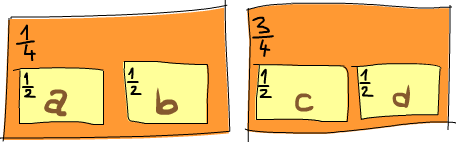
\includegraphics[width=0.8\textwidth]{\subfix{./images/prob.png}}
\end{figure}

这种情况的概率列表的表达式:

\begin{lstlisting}[language=Haskell]
  thisSituation :: Prob (Prob Char)
  thisSituation =
    Prob
      [ (Prob [('a', 1 % 2), ('b', 1 % 2)], 1 % 4),
        (Prob [('c', 1 % 2), ('d', 1 % 2)], 3 % 4)
      ]
\end{lstlisting}

注意它的类型是\acode{Prob (Prob Char)}。那么现在要考虑该如何打平一个嵌套的概率列表了,一旦逻辑成立,\acode{>>=}也就是\acode{join (fmap f m)},
即得到了一个单子。以下是一个\acode{flatten}来完成这件事:

\begin{lstlisting}[language=Haskell]
  flatten :: Prob (Prob a) -> Prob a
  flatten (Prob xs) = Prob $ concatMap multAll xs
    where
      multAll (Prob innerxs, p) = map (B.second (p *)) innerxs
\end{lstlisting}

与原文不同之处在于\acode{concat \$ map}被\acode{concatMap}代替,且\acode{\\(x, r) -> (x, p * r)}被简化成\acode{(Data.Bifunctor.second (p *))}。
函数\acode{multAll}接受一个概率列表,需要将列表里面的概率都乘以\acode{p},返回一个新的概率列表。将\acode{multAll}映射到了概率列表时,即成功的打平了列表。

现在来定义\acode{Monad}实例:

\begin{lstlisting}[language=Haskell]
  import Data.Bifunctor qualified as B
  import Data.Ratio

  instance Functor Prob where
  fmap f (Prob xs) = Prob $ map (B.first f) xs

  flatten :: Prob (Prob a) -> Prob a
  flatten (Prob xs) = Prob $ concatMap multAll xs
    where
      multAll (Prob innerxs, p) = map (B.second (p *)) innerxs

  instance Applicative Prob where
    pure x = Prob [(x, 1 % 1)]
    Prob fs <*> Prob xs = Prob $ [(f x, p * q) | (f, p) <- fs, (x, q) <- xs]

  instance Monad Prob where
    m >>= f = flatten (fmap f m)

  instance MonadFail Prob where
    fail _ = Prob []
\end{lstlisting}

与原文不同之处在于,GHC 7.10 之后\acode{Monad}的 superclass 是\acode{Applicative},因此需要实现\acode{instance Applicative Prob},详见
\href{https://wiki.haskell.org/Typeclassopedia#Definition_3}{Haskell Wiki}。对于实现\acode{Applicative}的\acode{<*>}可以参考十一章的
\acode{instance Applicative []},即\acode{fs <*> xs = [f x | f <- fs, x <- xs]}。具体来讲\acode{fs}是一个函数列表,\acode{xs}为值列表,
通过列表表达式将每个函数\acode{f}应用至每个值\acode{x}。那么在这里同理,\acode{Prob fs}是一个函数的概率列表,\acode{Prob xs}是一个值的概率列表,
\acode{(f, p) <- fs}则是解构每个函数概率列表中的元素为\acode{f}函数与\acode{p}概率,而\acode{(x, q) <- xs}则是解构每个值概率列表中的元素为
\acode{x}值与\acode{q}概率,然后将解构出来的函数\acode{f}应用至值\acode{x},两个概率\acode{p}与\acode{q}相乘,最后得到新的元组所构成的概率列表。
还有一点不同的在于\acode{fail}现在要单独实现在\acode{MonadFail}上。

那么我们现在有了一个单子,那么我们可以用它做什么?好吧,它可以帮助我们计算概率,我们将概率事件的值视为带有 context,而概率单子可以确保这些概率能在最终的
计算中反映出来。

假设我们有两个普通硬币以及一个灌铅的硬币,后者在十次抛掷中有九次会出现正面,那么一次性丢这三个硬币,有多大的概率会出现三个正面呢?

\begin{lstlisting}[language=Haskell]
  data Coin = Heads | Tails deriving (Show, Eq)

  coin :: Prob Coin
  coin = Prob [(Heads, 1 % 2), (Tails, 1 % 2)]

  loadedCoin :: Prob Coin
  loadedCoin = Prob [(Heads, 1 % 10), (Tails, 9 % 10)]
\end{lstlisting}

接下来是投掷三个硬币:

\begin{lstlisting}[language=Haskell]
  import Data.List (all)

  flipThree :: Prob Bool
  flipThree = do
    a <- coin
    b <- coin
    c <- loadedCoin
    return (all (== Tails) [a, b, c])
\end{lstlisting}

测试:

\begin{lstlisting}[language=Haskell]
  ghci> getProb flipThree
  [(False,1 % 40),(False,9 % 40),(False,1 % 40),(False,9 % 40),
   (False,1 % 40),(False,9 % 40),(False,1 % 40),(True,9 % 40)]
\end{lstlisting}

同时出现正面的机率是四十分之九,差不多是 25\% 的机会。单子并没有办法 join 所有都是 False 的情形,即所有硬币都是出现反面的情况。不过那不是个严重的问题,
可以写个函数来将同样的结果变成一种结果。以下是用于聚合\acode{Prob Bool}的函数,返回值\acode{(Rational, Rational)}是一个分别代表正确概率与错误概率
的元组:

\begin{lstlisting}[language=Haskell]
  getJoinedProb :: Prob Bool -> (Rational, Rational)
  getJoinedProb = foldr (\(x, p) (accT, accF) -> if x then (accT + p, accF) else (accT, accF + p)) (0, 0) . getProb
\end{lstlisting}

测试:

\begin{lstlisting}[language=Haskell]
  ghci> getJoinedProb flipThree
  (9 % 40,31 % 40)
\end{lstlisting}

\end{document}
